\documentclass{ctuthesis}

\ctusetup{
	xdoctype = B,
	xfaculty = F3,
	mainlanguage = english,
	titlelanguage = english,
	title-english = {Expedition scheduling in an automated warehouse},
	title-czech = {Rozvrhování vyskladňování z automatizovaného skladu},
	specification-file = {zav_prace.pdf},
	front-specification = true,
	department-english = {Department of Computer Science},
	author = {Jan Kalina},
	supervisor = {Ing. Martin Schaefer},
	supervisor-address = {Unknown,\\ Zářivá 232,\\
	  12000 Praha 2},
	  day = 13,
	month = 5,
	year = 2019,
	keywords-english = {scheduling, automated warehouse, optimization, simulation},
}

\ctuprocess

\begin{thanks}

TBD
\end{thanks}

\begin{declaration}

Prohlašuji, že jsem předloženou práci vypracoval
samostatně a že jsem uvedl veškeré použité informační zdroje v souladu
s Metodickým pokynem o dodržování etických principů při přípravě vysokoškolských
závěrečných prací.
\medskip


V Praze, \ctufield{day}.~\monthinlanguage{second}~\ctufield{year}

\end{declaration}
\begin{abstract-english}
This thesis deals with optimization problem of expedition scheduling in an automated warehouse with given set of parameters, requirements and set of items to dispatch in a day. Relevant scheduling problems and their solutions are discussed. Optimization method and objectives are then proposed for the given type of an automated warehouse. Proposed method is implemented in provided simulation tool and evaluated based on it's performance in the simulation.

\end{abstract-english}



\begin{abstract-czech}
test \ldots
\end{abstract-czech} 

\begin{document}

\maketitle

\chapter{Introduction}

Scheduling is a well studied and practical topic. It is widely used in manufacturing facilities, warehouses, which are discussed in this thesis, and many other industries where proper scheduling can play a great role in their success. Despite its importance and years of research, scheduling is quite a challenging problem, especially when it comes to real-world problems where finding an optimal schedule is usually nearly impossible due to its high computational complexity. 

Since the beginning of research in scheduling, many methods and approaches were developed for finding schedules close to optimal schedule in a reasonable time, but what is a good or optimal schedule? Determining the objective of a schedule is a problem on its own. The usual objective of scheduling is to minimize the makespan, which is the length of a schedule, but this objective alone is not sufficient because of the stochastic nature of real-world problems and customized requirements some facility may demand. Many facilities demand different and complex objectives. For example, in case of an automated warehouse, it may be crucial to not only finish expedition in required time but to also expedite items in required order. 

In this thesis, general methods for solving scheduling problems relevant to scheduling a daily expedition of the given automated warehouse configuration are discussed. Then, method and an objective of a schedule for the given automated warehouse and scenario is proposed and finally proposed method is implemented and evaluated based on results from the provided simulation tool. Basic structure and functionality of an automated warehouse were provided and are described in the upcoming section.

\section{The automated warehouse}

There are many different types of automated warehouses with very different requirements, structures and functionality. Problem of scheduling an expedition can be very different based on the structure and the type of an automated warehouse. In this thesis we consider one of the structures of automated warehouses that is fairly common and is based on real-world problem. 

\subsection{Description}
\label{subsec:Description}
The automated warehouse is part of a factory that produces some items. These items are stored in its warehouse and can be expedited. The automated warehouse has given number of aisles. Each aisle has racks on each side, where items are stored and on each aisle operates a single stacker crane. On one side of each aisle are connected two conveyors. The first conveyor is moving items from an aisle to one of the expedition ramps, where trucks can be loaded, and the second is bringing in items from production. Before each item reaches an expedition ramp, it needs to be processed by a scanner, which is located at the end of the first conveyor.

When a truck arrives at expedition ramp, stacker cranes should start unloading items on conveyor leading to the expedition ramp. Stacker cranes can move vertically and horizontally in an aisle and are able to hold a single item each. Stacker crane which has the requested item in its aisle moves to the item, grabs it and put it on the conveyor. In case of item arriving from production to an aisle. Stacker crane on that aisle should take this item and store in in a free position in the aisle. Stacker cranes operate automatically and either react to an item arrival from production or execute scheduled unloadings. If an item arrives from production, stacker cranes prioritize storing an item. It means that as soon as a stacker crane finishes action in progress it stores an item from a production even if it means delaying scheduled unloadings.

Additional details are stated in \ref{sec:Automated warehouse}.

\begin{figure}
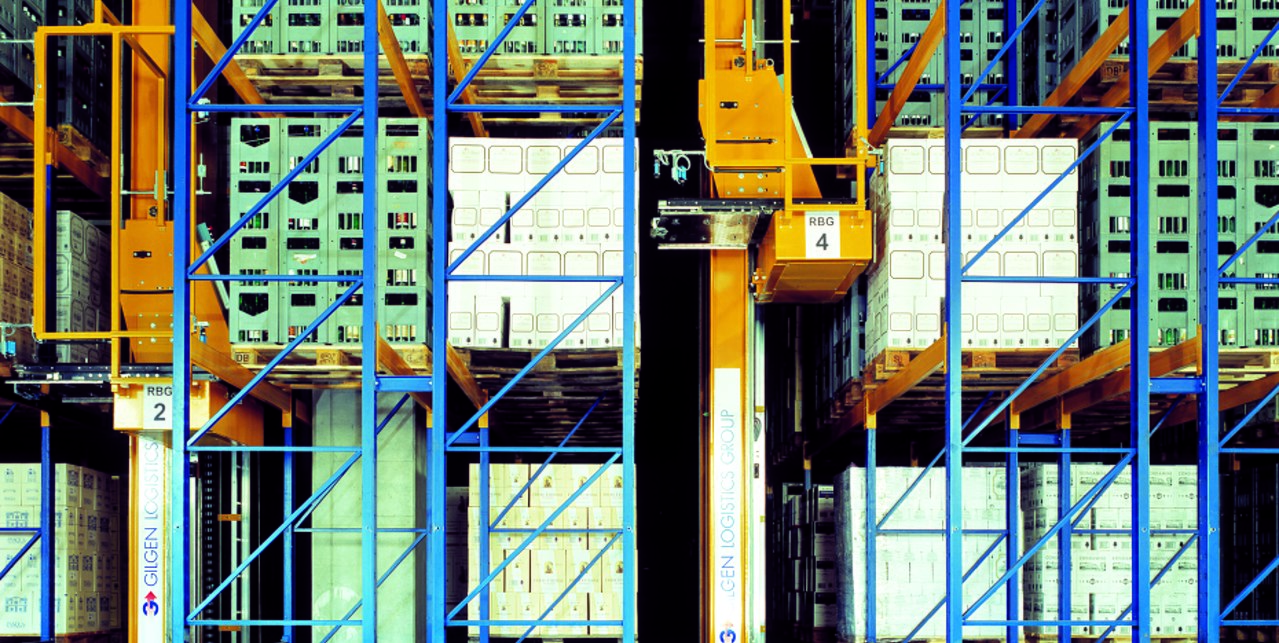
\includegraphics[width=0.8\linewidth]{highbaywarehouse.jpg}
\caption{Example of an automated warehouse with stacker cranes}
\label{fig:foobar}
\end{figure}

\section{Motivation}

Goal of this thesis is to be able to create appropriate schedule in reasonable time for the given automated warehouse and integrate this schedule to provided simulation tool so that the created schedule can be observed in action and evaluated based on it. With a combination of the schedule and the simulation tool, we are also able to get data about capabilities of the warehouse itself, which is valuable information when designing an automated warehouse. Integration of the scheduler to the simulation tool also enriches the simulation tool and can be used in future projects.

Properties to consider are prioritization of production handling, limited throughput and robustness to failure of individual robots. 

\section{Structure of this thesis}



\chapter{Problem statement}
\section{Automated warehouse}
\label{sec:Automated warehouse}
To be able to properly state scheduling problem. We need to specify some details on top of description in \ref{subsec:Description} and the way daily expedition work.

\subsection{Details of the automated warehouse}

Scanners, which are located at the end of every expedition conveyor, accepts an item periodically. Since scanner is processing items in given interval, there has to be space between items on conveyor based on the speed of the conveyor and the duration of the interval. If many items arrive too soon after each other, they pile up and may cause conveyor to stop, which should never happen. To prevent stopping of and conveyor, there is a small buffer. Number of items that pile up in the buffer during a daily expedition will be one of the measurements of robustness to delays.

We also simplify our problem and assume that workers at loading ramp can always pick up an item coming from scanner. This mean that scanners then create bottlenecks for each expedition ramp where throughput is limited by frequency at which scanner can process items.

\subsection{Expedition scenario}
We consider expedition is spanned over part of a one day. During expedition, a truck can arrive at the expedition ramp at scheduled time and demand certain number of items of different types, where items of different types are loaded in specified order. Which specific items will be expedited is known in advance and is expected that these items are distributed nearly equally. Stacker cranes then should be able start unloading demanded items, also at scheduled times. This process repeats throughout the expedition duration. 

\subsection{Available information}
Several basic parameters provided for the given automated warehouse. These parameters include horizontal and vertical speeds and accelerations of stacker cranes, dimensions of a warehouse, speed and length of conveyors, duration of scanning an item, duration of grabbing an item from a conveyor, duration of putting an item on a conveyor and exact location of each item stored in the warehouse. For expedition, we know count, types and order at which items should be loaded for each truck. 

From these parameters we are able to calculate data needed for describing machine scheduling model.

\section{Notation}*

\noindent \textbf{Job} ($job_i$) A $job_i$ represents an item $i$ to be expedited. Since expedition items are known in advance $job_i$ is already associated with one of the stacker cranes. 

\noindent \textbf{Machine} ($m_i$) A $m_i$ represents a stacker crane or a scanner. 

\noindent \textbf{Machine processing time} ($p_i$) Time which machine associated with $job_i$ needs to process $job_i$. In other words, time needed to unload an item $i$ from it's location to conveyor. This action consists of trip from conveyor to the item $i$, grabbing the item, trip back to conveyor and putting the item on it. Values of $p_i$ is calculated from speeds, accelerations and dimensions of the warehouse, but if production handling is taken into consideration, these values can become quite inaccurate since stacker crane may not always be at the same spot at the start of a job processing. Processing time is never zero.


\noindent \textbf{Scanning interval} ($s$) Processing time of a scanner. It is equal for every job.

\noindent \textbf{Traverse duration} ($t_i$)

\noindent \textbf{Completion time} ($c_i$)

\noindent \textbf{Start time} ($s_i$)

\noindent \textbf{Stacker crane completion time} ($scc_i$)

\noindent \textbf{Stacker crane start time} ($scs_i$)

\noindent \textbf{Position in expedition} ($pos_i$)

\noindent \textbf{TBD - expedition list, ... Add when needed} ($something_i$)


\section{Scheduling problem}
 
 Problem of expedition scheduling in the automated warehouse can be separated into two problems. The first problem is dealing assignment of a ramps to trucks and order of trucks at which they arrive. The second problem occurs after the first problem and it deals with assignment of completion times to jobs only, since machines are predetermined. This thesis mostly tackles the second problem since a good solution to the first problem is fairly easy to get as is shown in chapter 3 or 4?* and scheduling of the second problem has bigger effect on overall quality of the schedule.
 
 \subsection{Scheduling trucks}
 
 This problem can be described as parallel machine model.
 
 There are $m$ ramps in parallel and $n$ trucks planned for a day. Ramps can be interpreted as machines in parallel and jobs as whole expedition of each truck. Since each ramp includes only one scanner, which acts are bottleneck in the warehouse, objective of this problem should be to minimize makespan which often leads to good utilization of machines [pinedo]*.
 
\subsection{Expedition in the automated warehouse as machine scheduling model}

Problem of assigning completion times to jobs in the automated warehouse can be formulated as special case of 2-stage flexible flow shop (FF2) with blocking or flexible flow line (FFL) with two stages as follows:

There are 2 work stations connected in series. The first work stations consists of $m$ machines (stacker cranes) in parallel and the second work station consists of $l$ machines (scanners) also in parallel. Every job $job_i$ needs to be processed on it's predetermined machine. After job $job_i$ is processed, it travels to a scanner where it needs to be processed too. Jobs cannot wait between work stations and machines need to start processing a job as soon as it arrives. This alone is referred to as FFL.

Main requirements of this problem is make a schedule that fits into working hours of the warehouse and make the schedule robust to random events, i.e. arrival of an item from production can postpone scheduled job at a machine for a whole duration of storing the item and that can lead to loading items in wrong order and filling buffer at a scanner. In thesis objective of this problem is described as minimization of sum of weighted sub objectives, which are: Lateness, sum of idle times and standard deviation if idle times. These objectives were selected mostly based on reading on objective functions and robustness in [pinedo]*. Experimenting with these objectives and their effect is shown in chapter 5*.

Assuming objective function is linear, we can formulate this problem with single expedition ramp as linear program as follows:
\\

\textbf{Decision variables}

\begin{itemize}
\item $x_{ij}$: 1 if $job_i$ expedited immediately after $job_j$, 0 otherwise
\item$c_i$: completion time of $job_i$ on the second stage
\item$idle_i$: idle time followed after $job_i$ on the second stage
\item$y_i$: order number of $job_i$ on the second stage
\item$scc_i$: start time of $job_i$ on the first stage 
\end{itemize}
\textbf{Data}
\begin{itemize}
\item$p_i$: processing time of $job_i$ on the first stage
\item$E_i$: set of allowed order numbers on the second stage for $job_i$
\item$I_i$: set of indexes of jobs scheduled on machine $i$ on the first stage
\item$M$: represents a large number
\item$start$: time at which work hours start
\item$end$: time at which work hours end
\end{itemize}

\begin{equation}
\begin{aligned}
&\text{minimize}
&&f(\ldots)
\end{aligned}
\end{equation}
\begin{equation}
\begin{aligned}
\text{subject to}\\
& \sum_{i=0}^{n} x_{ij} = 1 && \text{for}\; i = 1, \ldots, n\\
& c_{i} - c_{j} + M(1 - x_{ij}) \geq s + idle_{i} && \text{for}\; i,j = 1, \ldots, n\\
& c_{i} - scc_{i0} = p_{i} + t_i + s + idle_i && \text{for}\; i = 1, \ldots, n\\
& scc_{i} + p_i < scc_j + M(1 - x_{ij}) && k = 0,\ldots,n, i,j \in I_k\\
& y_{i} - y_{j} < c_i - c_j + M(1 - x_{ij}) && \text{for}\; i,j = 1, \ldots, n\\
& y_i \in E_i && \text{for}\; i = 1, \ldots, n\\
& x_{ij} \in \{0, 1\}  && \text{for}\; i,j = 1, \ldots, n\\ 
& c_i \geq start && \text{for}\; i = 1, \ldots, n\\
& c_i \leq end && \text{for}\; i = 1, \ldots, n\\
& scc_{i} \geq start - p_i && \text{for}\; i = 1, \ldots, n\\
& idle_i \geq 0 && \text{for}\; i = 1, \ldots, n\\
\end{aligned}
\end{equation}

\chapter{Related work}

\section{Overview of methods and approaches for finding optimal schedule}
Problems are hard. Methods like b\&b, csp, mit, etc. should be used.
\section{Value of finding optimal solution}
Finding optimal solution is not really worth it in real world problems. Furthermore solving these problems with CSP or MIT requires too much processing time. Even in literature they are saying that around 50 jobs is the limit. 
\section{Solving scheduling problems in practice}
In practice solution is usually constructed using some simple heuristics. Complex heuristics is not really worth using because of random events. Questions usually is what should I try to improve and what heuristics should be good for that. 

FFLL 
\chapter{Proposed solution for our problem}
\section{Constraint satisfaction problem formulation}
\section{Algorithm description}
Heuristic construction algorithm

1. Truck allocation

First of all, trucks are distributed to ramps to achieve good utilization. There are some heuristics for this, but this task can be solved using MIP.

2. Order of jobs + dispatching

Using hybrid cyclic heuristics we can distribute jobs quite equally among machines and also try to minimize makespan or other objectives

3. Distribute available time as idle times

Now that we know how long is schedule, we can tell how much time we have until work hours end. We can take this time a distribute it among items as idle times. We cannot just simply postpone jobs by idle time, we have run step 2. again, now with idle times.

\section{Meta-heuristics}
Local search (Tabu, simulated annealing)

In scenario where we have more than one ramp, it's not easy to tell how much time I can distribute as idle time. Simulated annealing with ordered moves is good for distributing idle times among jobs. It can basically replace step 3 of proposed algorithm if it wasn't slower. It's better to use it after step 4 to distribute small timeslots to take advantage of remaining time of expedition.

Another improvement is using tabu search which swaps order number of two items. Some objectives are not easily minimized using some heuristics in step 2 like for example weighted penalty for scheduling two jobs right after each other on a single machine because it can lead to stopping a production

\chapter{Implementation}
\section{Simulation environment}
\section{Scheduler module}
\chapter{Evaluation}
\section{Performance}
\section{Scenarios}
\section{Comparison}
\subsection{Comparison of plan and behavior in simulation}
Comparing different version (LS, no LS, heuristic 1, heuristic 2, ...) of algorithm too.
\subsection{Effect of objectives?}
Mainly significance of idle times (at scanner or machines)
\chapter{Conclusion}

Lorep ipsum \cite{doe}

\begin{thebibliography}{1}

\bibitem{doe} J. Doe. \emph{Book on foobar.} Publisher X,
 2300.

\end{thebibliography}

\end{document}

